\documentclass[14pt]{beamer}
\title[JPL:Java:02]{JPL :: Introduction Arrays}
\author[TS]{TalentSprint}
\institute[L\&D]{Licensed To Skill}
\date{Version 1.0.4}
\usefonttheme{serif}
\usecolortheme{orchid}
\usepackage{bookman}
\usepackage{hyperref}
\usepackage[T1]{fontenc}
\usepackage{graphicx}
\usepackage{listings}
\graphicspath{{../../Images/}}
\beamertemplateballitem
\usebackgroundtemplate{
\includegraphics[width=\paperwidth]{TS-XP-Logo.jpg}}
\lstset{language=Java,numbers=left, numberstyle=\tiny, basicstyle=\footnotesize, numbersep=10pt, showstringspaces=false, breaklines=true,keepspaces=true, columns=flexible}
\begin{document}

\begin{frame}
  \titlepage
\end{frame}

\begin{frame}{Learning Objectives}
By the end of this presentation, you will be able to:
\begin{itemize}
\item Understand how to declare Arrays.
\item Learn how to initialize Arrays
\item Understand how to read Data from an Array
\item Understand how to manipulate Array Data
\end{itemize}
\end{frame}

\begin{frame}[fragile]{Introduction Arrays}
Let us recollect the Java program that adds four numbers.
\begin{lstlisting}[numbers=none]
public class SumExample {
    public static void main(String[] args) {
        int next, sumSoFar;
        next = Integer.parseInt(args[0]);
        sumSoFar = next;
        next = Integer.parseInt(args[1]);
        sumSoFar += next;
        next = Integer.parseInt(args[2]);
        sumSoFar += next;
        System.out.println("Sum: " + sumSoFar);
    }
}
\end{lstlisting}
\end{frame}

\begin{frame}[fragile]{Introduction Arrays}
\lstinline!java SumExample 25 35 50 40!
\begin{figure}[H]
\begin{center}
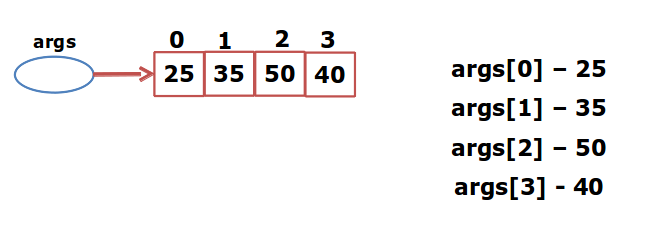
\includegraphics[scale=.45]{array-execution.png}
\end{center}
\end{figure}

\end{frame}

\begin{frame}{Introduction Arrays}
What is the meaning of args[0], args[1], args[2] etc. in the previous program?
\begin{itemize}
\item They are multiple pieces of data referred to by one variable named args and a corresponding index. These variables that hold more than one piece of data are called arrays in programming languages. 
\item Arrays are declared to hold a number of elements, and data is then written to and read from each element based on its index position.
\end{itemize}
\end{frame}

\begin{frame}[fragile]{Introduction Arrays}
\begin{block}{Declaring an Array Variable}
\begin{lstlisting}[numbers=none]
We can declare an array either of the following way.
<type>[] variable_name;
<type> []variable_name;
<type> variable_name[];
\end{lstlisting}
\end{block}
\begin{block}{Example}
\begin{lstlisting}[numbers=none]
int[] prime;
int []prime;
int prime[];
\end{lstlisting}
\end{block}
Array is not created at declaration and memory not allocated
\end{frame}

\begin{frame}{Introduction Arrays}
Defining  an Array

Unlike normal variables, an array needs to be defined before values can be assigned. When defined, memory will be allocated. An array is defined as:
variable\_name = new <type>[N];

Example: primes = new int[10];

Declaring and Defining in the same statement:
int[] primes = new int[10];

In the above examples, memory for 10 integers i.e. 40 bytes is allocated.
\end{frame}

\begin{frame}[fragile]{Introduction Arrays}
\begin{block}{Initializing an Array}
An array is initialized using loop.
\begin{lstlisting}[numbers=none]
for (i = 0; i < 10; i++)
    primes[i] = xxxxx;
\end{lstlisting}
\end{block}
\end{frame}

\begin{frame}[fragile]{Introduction Arrays}
\begin{block}{Initializing an Array}
Declaring, Defining and Initializing an array at the same time
\lstinline!int[] variable_name = {val1,val2,val3,...};!

Example: \lstinline!int[] prime = { 3,5,7,11,13,17,19,23,29};!

\end{block}
\end{frame}

\begin{frame}[fragile]{Introduction Arrays}
\begin{block}{Initializing an Array}
We can also initialize an array with an existing array:
    \lstinline!int[] even = {2,4,6,8,10};!
    \lstinline!int[] notOdd = even;!
\end{block}
One array but two array variables; both array variables refer to the same array; array can be accessed through either variable name.
\end{frame}

\begin{frame}[fragile]{Introduction Arrays}
\begin{block}{Try the following code and check the result.}
\begin{lstlisting}[numbers=none]
int[] primes = new int[20];    
primes[0] = 2;                   
primes[1] = 3;                   
int [] primes2 = primes;
System.out.println(primes2[0]);
primes2[0] = 5;
System.out.println(primes[0]);
\end{lstlisting}
\end{block}
\end{frame}

\begin{frame}[fragile]{Introduction Arrays}
Write a Java Program to declare, define, initialize and display an array.
\begin{lstlisting}[numbers=none]
public static void main(String[] args) {
    int[] myArray = new int[10];
    for(i=0; i<10; i++)
        myArray = i*2;
    for(i=0; i<10; i++)
        myArray = i*2;
}
\end{lstlisting}
\end{frame}

\begin{frame}[fragile]{Introduction Arrays}
Write a Java Program to search a value in an array 
\begin{lstlisting}[numbers=none]
public static void main(String[] arg) {
    int[] myArray = {23, 45, 12, 78, 27, 35, 67, 81};
    int key = Integer.parseInt(args[0]);
    for(i=0; i<10; i++) {
        if (key == myArray[i]) {
            System.out.print("Number found");
            return;
        }
    }
    System.out.print ("Number not found"); 		
}
\end{lstlisting}
\end{frame}

\begin{frame}{Introduction Arrays}
\small
\begin{enumerate}
\item Declare an integer array of size 10. Initialize using for loop with 1 to 10, and print all elements from an array.

\item Declare an integer array of size 10. Initialize using for loop with 1 to 10, use another for loop to calculate the sum of all integers of the array?

\item Declare an integer array of size 10. Initialize using for loop with 1 to 10, and print all elements from an array in reverse order.

\item Declare an integer array of size 10. Initialize using for loop with 1 to 10. Create another array of the same size and copy the first array into second in reverse order.

\end{enumerate}
\end{frame}

\begin{frame}{Introduction Arrays}
\small
Write a program for the following problem:

Jailer cell:
In Transum prison there are 100 prisoners in cells numbered 1 to 100.
On day 1, the guard turns the key in every lock to open every cell.
On day 2, the guard turns the key in every cell which is a multiple of 2. This locks all the even numbered cells.
On day 3, the guard turns the key in every cell which is a multiple of 3, locking or unlocking them.
This continues for one hundred days. The prisoners whose cells are open after the 100th day are set free.
Which prisoners will be set free? 
\end{frame}

\begin{frame}{Introduction Arrays}
\begin{figure}[H]
 \begin{center}
   
\includegraphics[scale=.3]{qa.png}   
 \end{center}
  \end{figure}
\end{frame}
\end{document}
